\documentclass{article}
\usepackage[T1]{fontenc}
\usepackage{lmodern}
\usepackage{graphicx}
\usepackage{amsmath,amssymb}
\usepackage[a4paper,margin=2cm]{geometry}
\usepackage[absolute,overlay]{textpos}
\setlength{\TPHorizModule}{1mm}
\setlength{\TPVertModule}{1mm}
\usepackage[indonesian]{babel}
\usepackage{hyperref}
\setlength{\emergencystretch}{2em}
% unit: Halaman 16

\begin{document}

% === Halaman 16 (llm) ===

\vspace{106.92mm}

\section*{Program Caesar Cipher dalam Bahasa Python}

\vspace{10mm}

% deskripsi: Screenshot cuplikan kode Python untuk fungsi Caesar\_cipher\_encrypt yang mengimplementasikan enkripsi Caesar Cipher.
% bbox normalisasi: [0.0400, 0.1600, 0.9300, 0.5200]
\begin{textblock*}{186.90mm}(8.40mm,47.52mm)
\noindent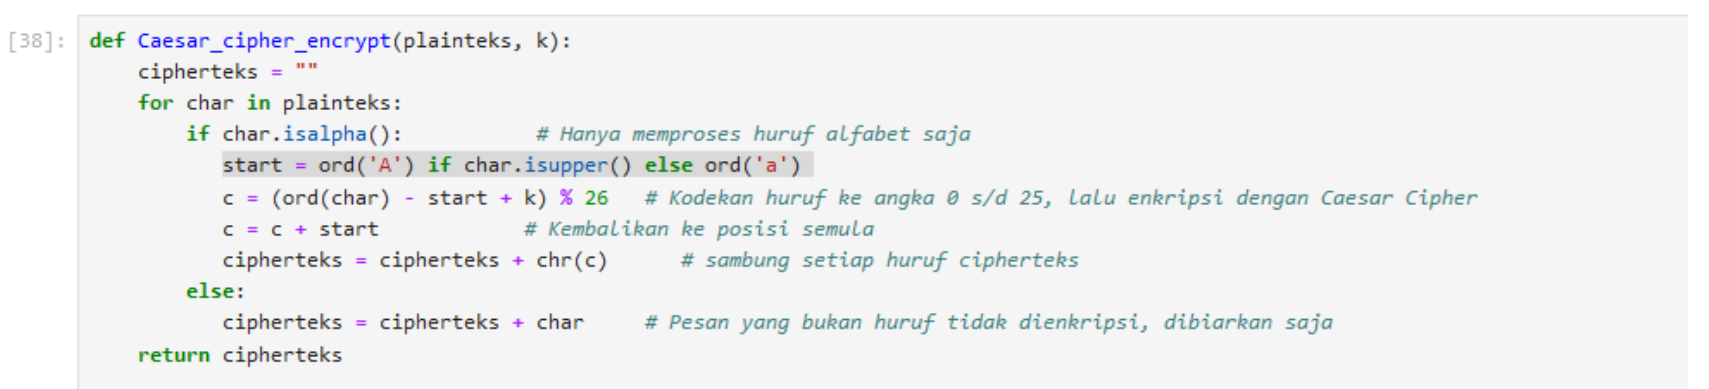
\includegraphics[width=186.90mm,height=106.92mm]{../../images/llm/page_016_img_01.png}%
\end{textblock*}

% deskripsi: Screenshot cuplikan kode Python untuk fungsi Caesar\_cipher\_decrypt yang mengimplementasikan dekripsi Caesar Cipher.
% bbox normalisasi: [0.0400, 0.5400, 0.9300, 0.9000]
\begin{textblock*}{186.90mm}(8.40mm,160.38mm)
\noindent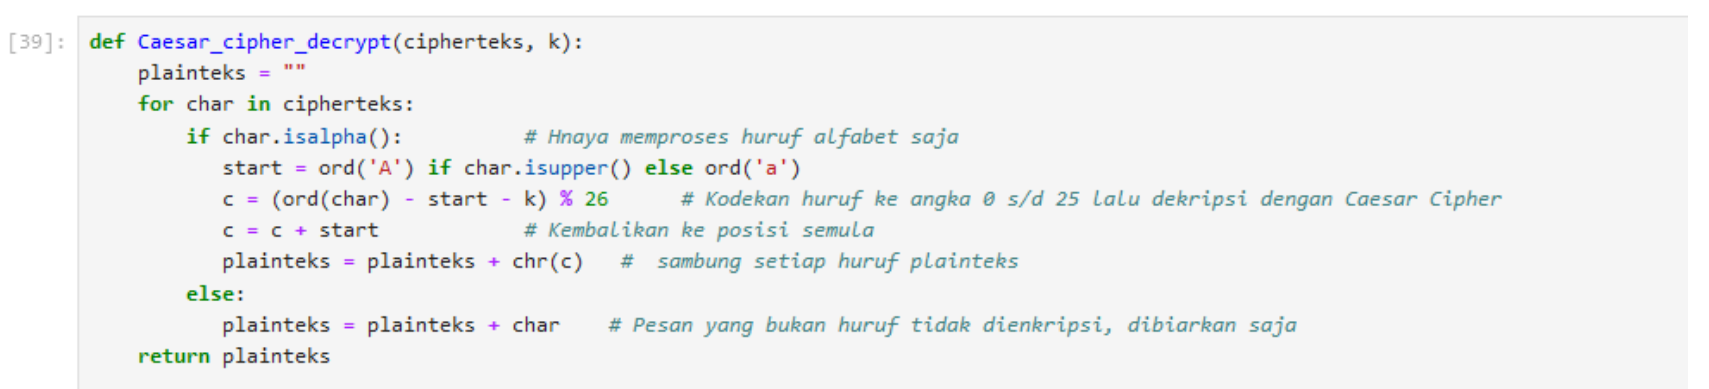
\includegraphics[width=186.90mm,height=106.92mm]{../../images/llm/page_016_img_02.png}%
\end{textblock*}

\end{document}
